\section{Relationale Algebra}

\begin{defi}{Relationale Algebra}
    Eine \emph{relationale Algebra} definiert (Mengen-)Operationen, die sich auf eine Menge von Relationen anwenden lassen.
    Damit können Relationen beispielsweise gefiltert, verknüpft oder aggregiert werden.
    Die Ergebnisse aller Operationen sind ebenfalls Relationen.
    Aus diesem Grund bezeichnet man die Relationenalgebra als abgeschlossen.

    Eine Relation
    \[
        R \subseteq D_1 \times \ldots \times D_n
    \]
    ist wie bisher primär eine konkrete Tupelmenge
    \[
        t = [a_1, \ldots, a_n] \in R, a_k \in D_k
    \]

    Eine Tabelle ist eine visuelle Repräsentation einer Relation und eine Zeile in einer Tabelle repräsentiert ein Tupel.

    Steht die Relation für einen Entitätstyp, so sind die Tupel konkrete Entitäten.
\end{defi}

\begin{bonus}{Funktionen zum Aufbau einer Relation}
    Ist man statt an einer Relation $R$, also der konkreten Tupelmenge, nur am Aufbau der Relation, d.h. den Attributen und Datentypen, interessiert, helfen diese Funktionen:
    \begin{itemize}
        \item $\ident(R) = \{a_i\}$
        \item $\schema(R) = \{[a_1:T_1, \ldots, a_n:T_n]\}$
    \end{itemize}
\end{bonus}

\begin{defi}{Schlüsselkandidat (Relationale Algebra)}
    Ein \emph{Schlüsselkandidat} $K$ mit $K \subseteq \ident(R)$ ist eine Menge von Attributen, deren Werte jeweils alle Tupel der Relation eindeutig identifizieren (\enquote{identifier}).

    So ist implizit garantiert, dass es keine zwei gleichen Tupel in der Relation gibt.

    Grundsätzlich kann es mehrere Schlüsselkandidaten geben, aus denen dann der Schlüssel (\enquote{primary key}) ausgewählt wird.
\end{defi}

\subsection{Mengenoperationen}

\begin{defi}{Voraussetzungen für Mengenoperationen}
    Um Mengenoperationen auf Relationen durchzuführen, müssen diese kompatibel sein.
    Das bedeutet, Attributanzahl und Wertebereiche müssen übereinstimmen (\emph{Vereinigungsverträglichkeit} bzw. \emph{Typkompatibilität}).

    Für zwei Relationen $S$ und $T$ muss also gelten, dass\footnote{Die Attribute müssen allerdings nicht formal gleich heißen, eine verträgliche Semantik ist aber sinnvoll.}
    \[
        \schema(S) = \schema(T)
    \]
\end{defi}

\begin{defi}{Klassische Mengenoperationen}
    Seien $S$ und $T$ zwei kompatible Relationen.
    Dann sind definiert:
    \begin{itemize}
        \item \emph{Vereinigung}:
              \[
                  S \cup T = \{ r \mid r \in S \lor r \in T \}
              \]
        \item \emph{Differenz}:
              \[
                  S - T = S \setminus T = \{ r \mid r \in S \land r \notin T \}
              \]
        \item \emph{Schnittmenge}:
              \[
                  S \cap T = \{ r \mid r \in S \land r \in T \}
              \]
    \end{itemize}

    Für mehr Informationen und Beispiele zu den konkreten Anwendungen in SQL: %\fullref{SQL}.
\end{defi}

\begin{defi}{Kartesisches Produkt}
    Für zwei Relationen $S$ und $T$ mit
    \[
        \ident(S) \cap \ident(T) = \emptyset
    \]
    ist das \emph{kartesische Produkt} $S \times T$ definiert durch
    \[
        S \times T = \bigcup_{(s_1, \ldots, s_n) \in S} \left[ \bigcup_{(t_1, \ldots, t_k) \in T} \{ (s_1, \ldots, t_1, \ldots, t_k) \} \right]
    \]

    Im üblichen kartesisches Produkt entstehen Paare $(s,t)$ mit $s \in S$ und $t \in T$.
    Hier hingegen entstehen $\abs{S \times T} = \abs{S} \cdot \abs{T}$ Tupel, bestehend aus allen Attributen einer Entität $s \in S$ verbunden mit den Attributen einer Entität $t \in T$.

    Im Fall $\ident(S) \cap \ident(T) = \emptyset$ würde obige Definition doppelte Attribute erzeugen, was mathematisch ein Problem ist, aber in der Praxis durch Umbenennung der Attribute gelöst werden kann.

    \emph{Eselsbrücke}: Jedes Element von $S$ mit jedem von $T$.
\end{defi}

\begin{defi}{Selektion}
    Für eine Relation $S$ und eine logische Bedingung $\Theta$ ist die \emph{Selektion} definiert durch
    \[
        \sigma_\Theta(S) = \{ s \in S \mid s \ \text{erfüllt} \ \Theta \}
    \]

    Selektionsbedingungen sind häufig Vergleichsoperationen ($=$, $\neq$, $\leq$, $<$, $>$, $\geq$) auf den Attributen und logische Verknüpfungen ($\land$, $\lor$, $\lnot$).

    Die Selektion wirkt wie ein Filter auf der Relation $S$, wo sie auf jedes Element angewandt wird.
\end{defi}

\begin{defi}{Projektion}
    Die \emph{Projektion} $\Pi_{a_{i1}, \ldots, a_{ik}}$ wählt aus einer Relation $S$ mit $\ident(S) = \{a_{1}, \ldots, a_{n}\}$ die Attribute $a_{i1}$ bis $a_{ik}$ aus:
    \[
        \Pi_{a_{i1}, \ldots, a_{ik}}(S) = \{ (a_{i1}, \ldots, a_{ik}) \mid a \in S \}
    \]

    Die mathematische Menge eliminiert Duplikate, die Ergebnismenge in SQL aber nicht.
\end{defi}

\begin{defi}{Theta-Join}
    Der \emph{Theta-Join} bzw. \emph{Theta-Verbund} $S \bowtie_{\Theta} T$ für zwei Relationen $S$ und $T$ und Selektionsbedingung $\Theta$ ist definiert durch
    \[
        S \bowtie_\Theta T = \sigma_\Theta (S \times T)
    \]

    Hier entstehen zunächst enorm große Datenmengen durch das kartesische Produkt, die dann durch die Selektion wieder reduziert werden.
    In der Praxis kann ein DBMS diese sehr häufigen Join-Operationen effizient durchführen.
\end{defi}

\begin{bonus}{Equi-Join}
    Der \emph{Equi-Join} ist ein Spezialfall des Theta-Join mit der Bedingung, dass der Inhalt bestimmter Attribute, z.B. $a_1$ und $a_2$, identisch sein muss, d.h. der speziellen Form $a_1 = a_2$ genügt:
    \[
        S \bowtie_{a_1 = a_2} T = \sigma_{a_1 = a_2} (S \times T)
    \]
\end{bonus}

\begin{defi}{Natural-Join}
    Ausgehend von der Idee, dass Primär- und Fremdschlüssel gleich heissen, nutzt der \emph{Natural-Join} dies aus und verbindet Entitäten, die in gleich benannten Attributen gleiche Werte besitzen\footnote{Also ein Equi-Join auf gleichen Attributen.}.

    Im Unterschied zum Theta-Verbund enthält der Natural-Join die gleichen Attribute nur einmal, eliminiert so also ungewünschte Redundanz.

    Für zwei Relationen $S$ und $T$ mit $\schema(S) = \{ [ a_1, \ldots, a_n, b_1, \ldots, b_k ] \}$ und $\schema(T) = \{ [ b_1, \ldots, b_k, c_1, \ldots, c_m ] \}$ ist der Natural-Join $S \bowtie T$ definiert durch\footnote{Das entspricht dem Schema $\{ [a_1, \ldots, a_n, b_1, \ldots, b_k, c_1, \ldots, c_m] \}$ und man sieht, dass die doppelten Attribute $S.b_i$ bzw. $T.b_i$ durch die Projektion $\Pi$ wegfallen.}
    \[
        S \bowtie T = \Pi_{a_1, \ldots, a_n, S.b_1, \ldots, S.b_k, c_1, \ldots, c_m} \sigma_{S.b_1 = T.b_1 \land \ldots \land S.b_n = T.b_n} (S \times T)
    \]

    \emph{Hinweis:}

    Von der Verwendung von Natural-Joins wird abgeraten!
    Beim Natural-Join werden immer alle gleichnamigen Attribute verwendet, d.h. Hinzufügen neuer Attribute oder Umbenennen vorhandener Attribute führt schnell zu einer Änderung der Abfrage.
\end{defi}

\begin{bonus}{Semi-Join}
    Wenn einen nur die Existenz, nicht aber die Attributwerte der assoziierten Entität $T$ beim (Natural-)Join interessiert, nutzt man den \emph{Semi-Join}.

    Der Semi-Join $S \ltimes T$ ist für zwei Relationen $S$ und $T$ definiert durch
    \[
        S \ltimes T = \Pi_{\ident(S)} (S \bowtie T)
    \]
\end{bonus}

\begin{bonus}{Anti-Semi-Join}
    Beim \emph{Anti-Semi-Join} $S \rhd T$ zweier Relationen $S$ und $T$ werden die Tupel aus $S$ selektiert, die am Natural-Join \emph{nicht} teilnehmen:
    \[
        S \rhd T = S - (S \ltimes T) = S - \Pi_{\ident(S)} (S \bowtie T)
    \]
\end{bonus}

\begin{defi}{Outer-Join}
    Ein \emph{Outer-Join} funktioniert im Grunde wie der Inner-Join.
    Im Kontrast dazu gibt er aber nicht nur die Datensätze beider Tabellen aus, die die Selektionsbedingung erfüllen, sondern zusätzlich auch alle übrigen Tupel der einen bzw. der anderen Tabelle.

    Bezogen auf die Leserichtung spricht man von einer linken und einer rechten Relation.

    Die jeweiligen Operationen heißen dementsprechend \emph{Left-Outer-Join} und \emph{Right-Outer-Join}.

    Bei einem Left-Outer-Join zweier Relationen $S$ und $T$
    \[
        S \lojoin T
    \]
    werden alle Entitäten der Entitätenmenge links der Relation, also $S$, berücksichtigt, auch wenn es keine zugehörigen Entitäten in Entitätenmenge $T$ gibt.
    Diese Attribute sind dann \texttt{NULL}.

    Bei einem Right-Outer-Join zweier Relationen $S$ und $T$
    \[
        S \rojoin T
    \]
    gilt das analog, nur mit vertauschten Rollen.

    Der \emph{Full-Outer-Join} zweier Relationen $S$ und $T$
    \[
        S \fojoin T
    \]
    ist die Vereinigung von Left- und Right-Outer-Join.
    Das bedeutet, es sind alle Entitäten beider Seiten dabei, nur ggf. mit \texttt{NULL}-Einträgen in den Attributen der anderen Seite, wenn es keine zugehörige Entität gibt.
\end{defi}

\begin{bonus}{Inner-Join vs. Outer-Join}
    \begin{center}
        \begin{tabular}{ccccccc}
            \underline{Inner-Join} & \quad                                                                                   & \underline{Left-Outer-Join} & \quad & \underline{Right-Outer-Join} & \quad & \underline{Full-Outer-Join} \\
            \\
            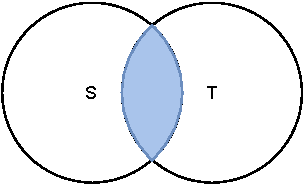
\includegraphics[width=0.2\linewidth]{includes/figures/bonus_join_inner_venn.pdf}
                                   & \quad
                                   & 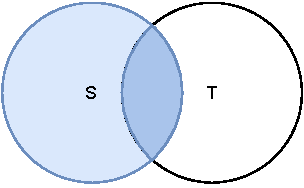
\includegraphics[width=0.2\linewidth]{includes/figures/bonus_join_outer_left_venn.pdf}
                                   & \quad
                                   & 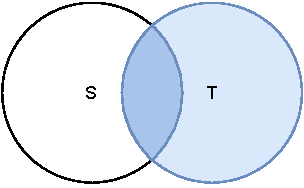
\includegraphics[width=0.2\linewidth]{includes/figures/bonus_join_outer_right_venn.pdf}
                                   & \quad
                                   & 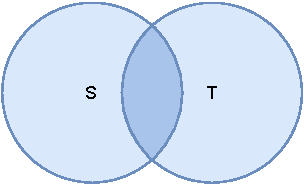
\includegraphics[width=0.2\linewidth]{includes/figures/bonus_join_outer_full_venn.pdf}
        \end{tabular}
    \end{center}
\end{bonus}

\begin{sql}{Differenz}
    Die \emph{Differenz} ist in MySQL bzw. MariaDB als Opesration so nicht vorhanden, kann aber leicht über Joins abgebildet werden.

    Für zwei Relationen $S$ und $T$ mit $\schema(S) = \schema(T)$ und Schlüsselattribut $K$ gilt:
    \[
        S - T \iff \text{\texttt{SELECT S.* FROM S LEFT OUTER JOIN T USING(K) WHERE isnull(T.K);}}
    \]
\end{sql}

\begin{sql}{Schnittmenge}
    Die \emph{Schnittmenge} ist in MySQL bzw. MariaDB als Operation so nicht vorhanden, kann aber leicht über Joins abgebildet werden.

    Für zwei Relationen $S$ und $T$ mit $\schema(S) = \schema(T)$ und Schlüsselattribut $K$ gilt:
    \[
        S \cap T \iff \text{\texttt{SELECT S.* FROM S JOIN T USING(K);}}
    \]
\end{sql}

\begin{defi}{Umbenennen von Relationen oder Attributen}
    Bei einem Join oder kartesischen Produkt kommt es zuweil vor, dass in der Ergebnisrelation eigentlich Attribute gleich heissen würden, was mathematisch und technisch ein Problem ist.
    Analog kann es notwendig sein, ganzen Relationen einen eigenen Namen zu geben, um etwa bei einem Self-Join diese zu unterscheiden.


    Zum \emph{Umbenennen von Relationen und Attributen} wird der Operator $\rho$ verwendet.
    Das Umbenennen einer Relation $S$ zu $S'$ wird dann mittels
    \[
        \rho_{S'}(S)
    \]
    und das Umbenennen eines Attributes $a$ zu $a'$ einer Relation T mittels
    \[
        \rho_{a \to a'}(T)
    \]
    notiert.
\end{defi}

\begin{defi}{Division}
    Für zwei Relationen $S$ und $T$ mit $\schema(S) = \{ [ a_1, \ldots, a_n, b_1, \ldots, b_k ] \}$ und $\schema(T) = \{ [ b_1, \ldots, b_k ] \}$ ist die \emph{Division} $S \div T$ definiert durch
    \[
        S \div T = \{ (a_1, \ldots, a_n) \mid \forall (b_1, \ldots, b_k) \in T : (a_1, \ldots, a_n, b_1, \ldots, b_k) \in S \}
    \]
    bzw. äquivalent
    \[
        S \div T = \Pi_{S-T}(S) - \Pi_{S-T}( (\Pi_{S-T}(S) \times T) - S )
    \]

    Die Division $\div$ ist also die \enquote{Umkehroperation} zum kartesischen Produkt, denn es gilt symbolisch:
    \[
        (S \times T) \div T = S
    \]

    \emph{Hinweis:}

    Die Ergebnismenge ist nur der $a$-Anteil von $S$, also $\Pi_a(S) = \Pi_{a_1, \ldots, a_n}(S)$.
\end{defi}

\begin{defi}{Aggregation und Gruppierung}
    Die \emph{Gruppierung} wendet \emph{Aggregatfunktionen}\footnote{Aggregatfunktionen sind z.B. \texttt{COUNT}, \texttt{AVG}, \texttt{SUM}, \texttt{MIN} und \texttt{MAX}.} auf gleiche Attribute in einer Relation an.

    Der Operator $\gamma$ erhält eine Liste von (Gruppierungs-)Attributen $a_1, \ldots, a_n$ und Aggregatfunktionen $f_1, \ldots, f_k$, die dann auf die Tupel angewendet werden, für die die Attribute der Attributliste gleich sind.

    Man schreibt für eine Relation $S$ dann
    \[
        \gamma_{a_1, \ldots, a_n; f_1, \ldots, f_k}(S)
    \]

    Jede Aggregatfunktion $f_1, \ldots, f_k$ ergibt eine Spalte in der Ergebnistabelle.
\end{defi}